\documentclass[11pt]{beamer}
\usepackage{verbatim}
\usepackage{amsmath}
\usepackage{amsthm}
\usepackage{multicol}
\usepackage{graphics}
\usepackage{color}
\usepackage{stmaryrd}\usefonttheme[onlymath]{serif}
\usepackage{CJK}
\title{Group Meeting - 1}
\date{\today}
\author{Presentor: Xie Li}
\begin{document}
\maketitle

\begin{frame}\frametitle{Overview}
\begin{itemize}
\item Interest of research and former projects.

\item Progress and problems last week.
\begin{itemize}
\item SMACK.
\item Memory model and points-to analysis.
\end{itemize}

\end{itemize}
\end{frame}

\begin{frame}\frametitle{Research Interests}

Program analysis and verification.
\begin{itemize}
\item Termination: ranking function.
\item Invariant synthesis: template-based, interpolant-based and abstract interpretation.
\begin{itemize}
\item How to find adequate interpolant.
\item ...
\end{itemize}
\item Memory safety: currently ongoing project which intends to participate SV-COMP.
\begin{itemize}
\item Survey on the frontend tool: SMACK.
\item Current Problems.
\end{itemize}
\end{itemize}
\end{frame}

\begin{frame}\frametitle{SMACK: Architecture}

SMACK is an front-end tool capable of converting source code like C into IVL Boogie via LLVM IR.

\textbf{Architecture of the toolchain:}

\begin{center}
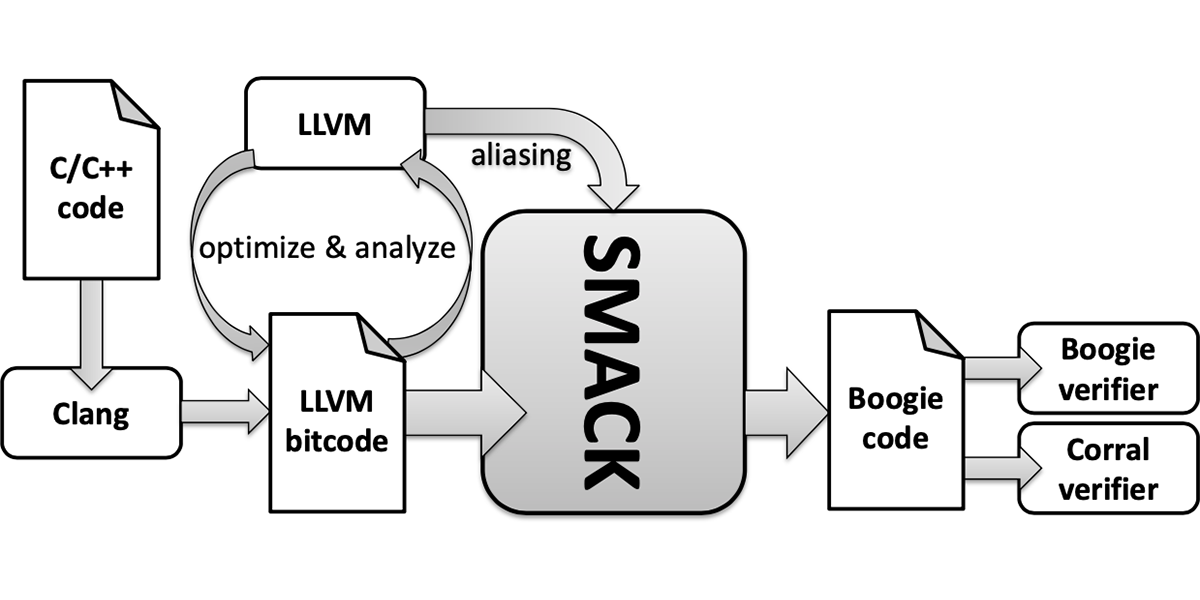
\includegraphics[scale=0.20]{smack_arch.png}
\end{center}
 


\end{frame}

\begin{frame}\frametitle{Problems for Memory Safety Program}
\begin{itemize}
\item How memory model involves in the verification? (The basic idea)
\item Separation logic? 

How to modify the assertion of boogie.
\end{itemize}


\end{frame}

\iffalse
\begin{frame}\frametitle{Process of the Transformation}
\textbf{From LLVM bitcode to Boogie IVL:}
\begin{enumerate}
\item  \texttt{createInternalizePass()},  \texttt{createDeadCodeEliminationPass()} and \texttt{RemoveDeadDefs()}.
\item \texttt{createRemovePtrToIntPass()}, \texttt{createLowerSwitchPass()} and Passes for loop unrolling.
\item \texttt{NormalizeLoops()}, \texttt{SimplifyEV,IV}, \texttt{createCodifyStaticInitPass()}...
\item \texttt{MemorySafetyChecker()}, \texttt{IntegerOverflowChecker()}.
\item \color{red}{\texttt{SmackModuleGenerator()}, \texttt{BplFilePrinter()}}.
\end{enumerate}


\end{frame}
\begin{frame}\frametitle{Introduction to the SMACK: A Demo Example}
C source code:
\begin{center}
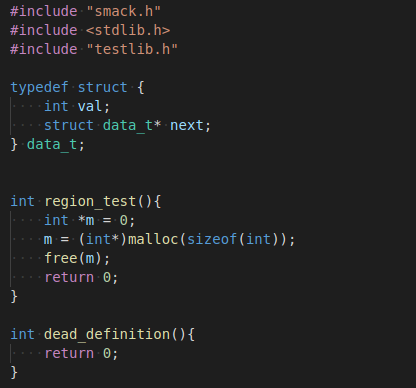
\includegraphics[scale=0.35]{example_code1.png}
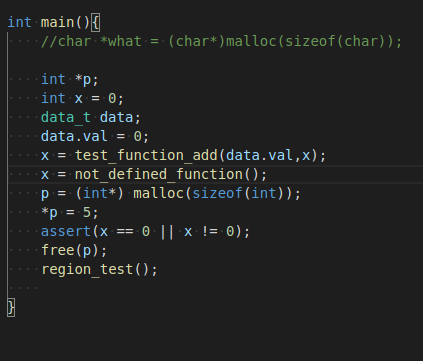
\includegraphics[scale=0.35]{example_code2.png}
\end{center}

\end{frame}

\begin{frame}\frametitle{LLVM IR}
\begin{center}
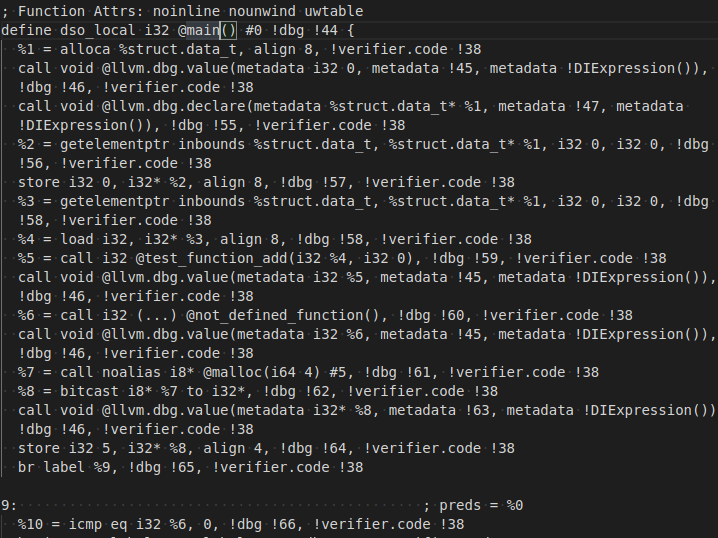
\includegraphics[scale=0.4]{llvm_ir_text.png}
\end{center}
\end{frame}

\begin{frame}\frametitle{Boogie IVL}
\begin{center}
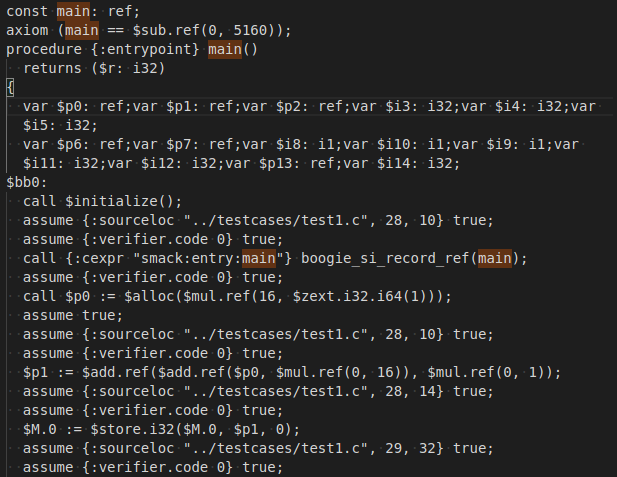
\includegraphics[scale=0.4]{boogie_main.png}
\end{center}
\end{frame}


\begin{frame}\frametitle{LLVM API}
LLVM API provides good support for developers on dealing with the optimizing and transforming of LLVM IR. In SMACK, before going through the passes, it first execute:
\begin{center}

\texttt{module = llvm::parseIRFile(InputFilename);}
\end{center}




\begin{itemize}
\item Module

\item Function

\item BasicBlock

\item Instruction
\end{itemize}

\end{frame}


\begin{frame}\frametitle{LLVM API}
LLVM API provides various preset passes:
\begin{itemize}
\item \texttt{llvm::createGlobalDCEPass()}
\item \texttt{llvm::createDeadCodeEliminationPass()}
\item \texttt{llvm::createLowerSwitchPass()}
\item \texttt{llvm::createLoopUnrollPass()}
\item ...
\end{itemize}

If we wish to use these passes later, the functionalities of these passes need to be specified later.

LLVM API also provides convienient interface for extension:

\begin{itemize}
\item \texttt{llvm::InstVisitor<SmackInstGenerator>}
\item \texttt{llvm::cl} for easy commandline argument manipulation.
\end{itemize}
\end{frame}


\begin{frame}\frametitle{A Program in Boogie AST}
\begin{definition}[Boogie Program]
A program in boogie IVL is sequence of declarations.
\end{definition}

On the implementation level: prelude $+$ a list of \texttt{Decl} object.

\begin{itemize}
\item 7 Kinds of \texttt{Decl}: \texttt{ConstDecl,TypeDecl,AxiomDecl, ConstDecl, VarDecl, CodeDecl, FuncDecl, ProcDecl}

\item \texttt{Stmt} are used in e.g. \texttt{FuncDecl}: \texttt{Assign, Assume, Assert, Goto, Code, Return, Call, Comment, Havoc}.
\item \texttt{Expr}, \texttt{Attr}..
\end{itemize}
\end{frame}


\begin{frame}\frametitle{A Coarse Mapping from LLVM IR to Boogie AST}

\begin{multicols}{2}
\begin{itemize}
\item Module
\item Function, BasicBlock
\item Instruction
\end{itemize}


\begin{itemize}
\item \texttt{Program}
\item \texttt{FuncDecl, CodeDecl..}
\item \texttt{Stmt}
\end{itemize}
\end{multicols}


\end{frame}


\begin{frame}\frametitle{Memory Model (No Reuse)}
\begin{itemize}
\item Address are integers.
\item One unbounded integer is stored at each address.
\item Heap addresses are allocated in a strictly increasing fashion.
\item Freed addresses are never reallocated.

\end{itemize}


\end{frame}

\begin{frame}\frametitle{Memory Model (No Reuse)}
\begin{itemize}
\item Address space partition (Address $A$):
\end{itemize}
\begin{multicols}{2}
\begin{itemize}
\item $A>0$
\item $A=0$
\item $\mathtt{GLOBALS\_BTM} \le A < 0$
\item $\mathtt{GLOBALS\_BTM} - 32768 \le A < \mathtt{GLOBALS\_BTM}$
\item $\mathtt{EXTERNS\_BTM}  \le A < \mathtt{GLOBALS\_BTM}- 32768$
\end{itemize}
\begin{itemize}
\item Heap
\item \texttt{NULL}
\item Static global storage
\item Padding
\item External global objects returned from external functions
\end{itemize}
\end{multicols}

A glimpse at the source here.


\end{frame}


\begin{frame}\frametitle{Transformation from LLVM IR to Boogie}
\color{red}{\texttt{SmackModuleGenerator}}: \color{black}A pass generating a Boogie program from a module by replacing the module of llvm into a list of declarations.

\color{red}{\texttt{SmackRep}}: \color{black}the class responsible for the replacement.


\begin{itemize}
\item \texttt{globalDecl}: generate global declarations according to IR, add constraints that global declarations are put in the \textbf{global storage}.

\item \texttt{ProcDecl}: insert a list of procedure declarations by replacing all functions in the module.

\item \texttt{SmackInstGenerator}: generate \texttt{Stmt} for each procedure generated above by iterating all the instruction in functions.

\item Generate prelude.
\end{itemize}

\end{frame}

\begin{frame}\frametitle{Generate Prelude}
A \texttt{Prelude} is initialized by a \texttt{SmackRep} object. The generation include:
\begin{itemize}
\item \texttt{TypeDeclGen}: create the declaration for some basic types in boogie. 
\item \texttt{ConstDeclGen}: create constant declaration for integer, pointers...
\item \texttt{MemDeclGen}: create memory regions.
\item \texttt{IntOpGen}
\item \texttt{PtrOpGen}
\item \texttt{FpOpGen}
\end{itemize}

Have a look at the corresponding with the source code.

\end{frame}

\begin{frame}\frametitle{\texttt{SmackRep}}
\begin{center}
\texttt{SmackRep(DataLayout*,Naming*,Program*,Regions*)}
\end{center}
\end{frame}

\begin{frame}\frametitle{Regions}
\begin{center}

Region: Node + Offset + Length
\end{center}

\begin{itemize}
\item A bunch of instructions involving pointers are visited. (\texttt{Region::idx}).

\item A region is created for the pointer operand (\texttt{Region::init}).

\item Merge the created region into existing one if they overlap. 
\end{itemize}
\end{frame}


\begin{frame}\frametitle{SMACK Header}
\begin{center}
\texttt{\#include "smack.h"}
\end{center}

\begin{itemize}
\item \texttt{\_\_SMACK\_} $+ $ \texttt{code, mod, decl, value...}
\item \texttt{\_\_VERIFIER\_} $+$ \texttt{assume, assert, nondet} 
\end{itemize}


\end{frame}

\begin{frame}\frametitle{Remaining Problems}

\begin{itemize}
\item No systematic way to specify the passes.
\item Details of instructions replacement need to be specified, especially those with 
\begin{itemize}
\item region operations,
\item assertion and assumption generation.
\end{itemize}
\item Figure out the intention of passes.
\item DSA, memory model..
\end{itemize}

\end{frame}


\fi
\end{document}